
\documentclass[twocolumn, amsmath]{revtex4}

\usepackage{graphicx}
\graphicspath{ {tex_pics/} }


\begin{document}


\title{PHYS 605 Lab \#6} 

\author{Morgan A. Daly}
\author{Evin O'Shea}
\date{\today} 


\maketitle


\section{Introduction and Theory}
\subsection{Purpose}

In this lab, the focus was to learn about how diodes can be used in AC circuits. The first part of the lab showed how a single diode can be used as a half-wave rectifier. In the second part of the lab the group made a full wave rectifier. In the third part of the lab the behavior of a zener diode was explored both with DC and AC voltage sources.

\subsection{Background / Theory}

The lab revolved around the behavior of diodes in AC circuits. Diodes are an interesting type of passive circuit element which have interesting properties. The most important property of diodes is that they only allow current flow in one direction. When an AC voltage source powers a diode, only the positive or negative voltage will go through the diode. 
%not sure where to put this if at all
%The second interesting property of diodes is that they have a minimum voltage required to pass current through/ has a max? clipps the voltage?

In the Part A of the lab a diode was used to convert the AC signal into only a positive signal. This demonstrated the diode property of only allowing current flow in one direction. When the AC source supplies a positive voltage the diode would allow current flow through. When the voltage source supplies a negative voltage the diode will not let current flow through. The circuit used for this part of the lab was built in two aprts. First the circuit was built with a resistor and a diode in series with the oscilliscope connected in parallel with the voltage source and the diode. After this circuit was investigated a 3V DC supply was added to the circuit between the resistor and diode. The final circuit for this part of the lab is shown below:

\begin{figure}
    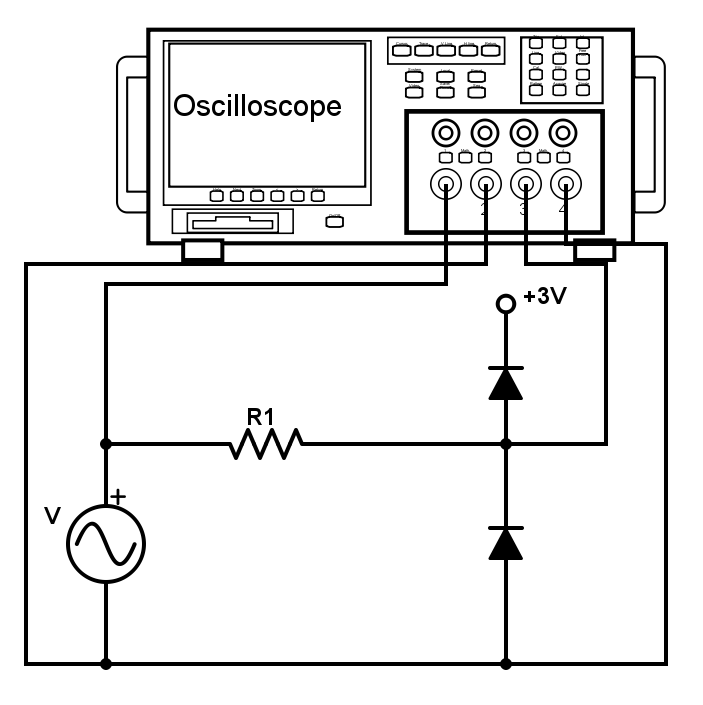
\includegraphics[scale=0.6]{halfwave.png}  
    \caption{This circuit only supplies postive voltage to the oscilloscope.}
\end{figure}

In the second part of the lab, the diode was used to allow the positive and negative voltages through while inverting the negative voltage. The circuit used for this part of the lab is shown below:

\begin{figure}
    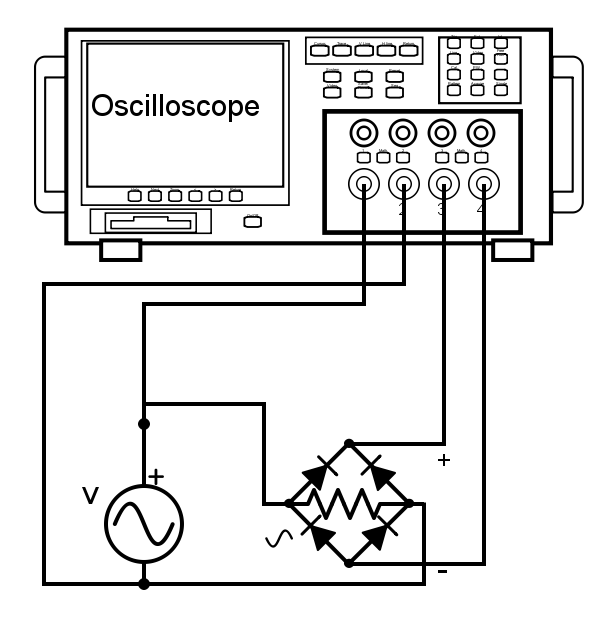
\includegraphics[scale=0.6]{bridge.png}  
    \caption{A full wave rectifier with input and output connected to an ocsilloscope}
\end{figure}

The circuit makes all the voltage positive. As positive voltage is supplied to the circuit current will pass through the top left diode and not the bottom left because of the orientation of the diode. Current will then flow down through the resistor and not the top right diode. As negative voltage is supplied to the circuit current will flow from the bottom side of the AC source. As the current flows to the right side of the bridge it will pass through the top right diode and not the bottom right. The current will then flow down through the resistor as it did when a positive voltage was supplied. This combination will cause flow in only one direction through the resistor and the output of the bridge.

For the third part of the lab, a zener diode was investigated. The distinction between a regular diode and a zener diode is that a zener diode will allow voltage to pass in both directions, but in the reverse-bias direction, there is a minimum voltage required to cause current flow. This voltage is called the zener voltage. A diagram of the circuit for this part of the lab is shown below:

\begin{figure}
    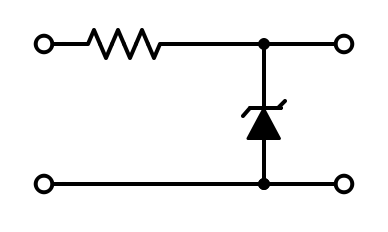
\includegraphics[scale=0.6]{zener.png}  
    \caption{This circuit only supplies postive voltage to the oscilloscope.}
\end{figure}

The left side was connected to both DC and AC sources to invesitage different properties of the zener diode. 


\begin{figure}
    \includegraphics[scale=0.6]{lab3circuit.png}  
    \caption{A circuit built so that the voltage across the capacitor, $v_C$, can be compared with the voltage from the source, $v_{in}$. The phase shift $\phi$ can also be observed.}
\end{figure}



\section{Methodology}

\begin{enumerate}
    \item Construct RC circuit with oscilloscope as show in figure (1).
    \item Adjust the circuit in order to gain some intuition about how the it behaves--- vary the resistor, frequency, and capacitor and note the effects. 
    \item Choose a circuit design such that a range of behavior can be observed while keeping the frequency below \SI{100}{\kilo\hertz}.
    \item Measure and record the voltage drop, $V_C$, and the phase shift with respect to input, $\phi_C$ across the capacitor. 
    \item Measure and record the voltage drop, $V_R$, and the phase shift with respect to input, $\phi_R$ across the resistor. 
    \item Repeat steps (4) and (5) for several (about ten) frequencies spanning multiple orders of magnitude.
\end{enumerate}


\section{Results and Analysis}

\subsection{Data}

3.065V (DC)
first amplitude/frequency: 2.64V  f=7.225Hz 
-V2(max) 1.78V

second amplitude: 4.08V f=7.225Hz
-V2(max) 2.72V

second frequency: 2.64V f=0.732Hz
-V2(max) 960mV

third frequency: 2.64V f=74.63Hz
-V2(max) 1.76V

fourth frequency: same for higher

WITH DIODE AND +3V

first: 2.64V 731.0mHz
V2 464mV

second: 2.64V  74.63Hz
V2 480mV

third: 1.48V f=7.225
v2 460mV

\end{center}


\subsection{Calculations}

The impedance of the capacitor, $Z_C$, and the impedance of the resistor, $Z_R$, could be calculated using equations (1) and (2).\\
$$Z_R(\omega)=\SI{10\,000}{\ohm}$$
$$Z_C(\omega)=\frac{1}{j \omega \,\, 4.7\times10^{-6} }$$
Using equation (6), the gain was calculated, first with the ratio of the voltages, then using the impedances where $Z_2$ was the impedance of the capacitor and $Z_1$ was the impedance of the resistor. This allowed us to calculate error.
\begin{center}
	\begin{ruledtabular}
    \begin{tabular}{ l  l  l l}
    f [Hz] & $Gain_{measured}$& $Gain_{expected}$ &  \% Error\\ \colrule
10.92&-10.4&-12.5	&  16.8 \\
24.04&-16.8&-18.17	&  7.53\\
71.73&-24.6&-26.9	&  6.92\\
97.66&-28.9&-29.5	&  2.03\\
337.8&-39.2&-40.1	&  2.24\\
757.4&-48.9&-47.0	&  4.68\\
1\,066&-48.9&-50.0	&  2.20\\
5\,102&-55.7&-63.6	&  12.4\\
12\,990&-57.6&-72.7	&  20.8\\
    \end{tabular}
    \end{ruledtabular}
\end{center}

 
\subsection{Analysis}

Observing the circuit's behavior qualitatively demonstrated that increasing resistance and decreasing capacitance causes an increase in the voltage across the capacitor. It also showed that a change in capacitance will change the phase shift, but a change in resistance will not.

The variation in error for the attenuation suggests that a substantial portion of the error was due to the oscilloscope. There was also more error at the lowest frequencies and highest frequencies. This could be due to less accurate measurements being made when the voltage across the capacitor was very small.

\begin{figure}[h]
    \includegraphics[scale=0.24]{bode}
    \caption{A Bode plot of the data. The measured values are in blue, while the expected values from equations (6) and (7) are in red.}
\end{figure}

Using the data collected, a Bode plot was drawn. It is apparent that all of the measured values are after the so-called ``-3 dB Point" as the gain plot is definitively negative.

The phase shift plot seemed slightly more erratic. Because the plot is after the -3 dB point, it is expected that the phase will begin to approach $90^\circ$.

A line was fit to the gain plot, and the slope showed that the roll off of the transfer function is 16.24 dB/decade. 


\section{Conclusion}
The relationship between frequency, impedance, and voltage was made obvious, and observations matched expectations based on known equations. The resulting improved understanding and intuition for a new type of circuit makes this successful.

Measured values of gain were compared to calculated values with some error, which seemed to increase at extreme values. The roll off was calculated, and the group was able to observe the behavior of a RC circuit in frequencies that were a part of the filtered frequencies.

\end{document}

